

\tikzset{every picture/.style={line width=0.75pt}} %set default line width to 0.75pt        

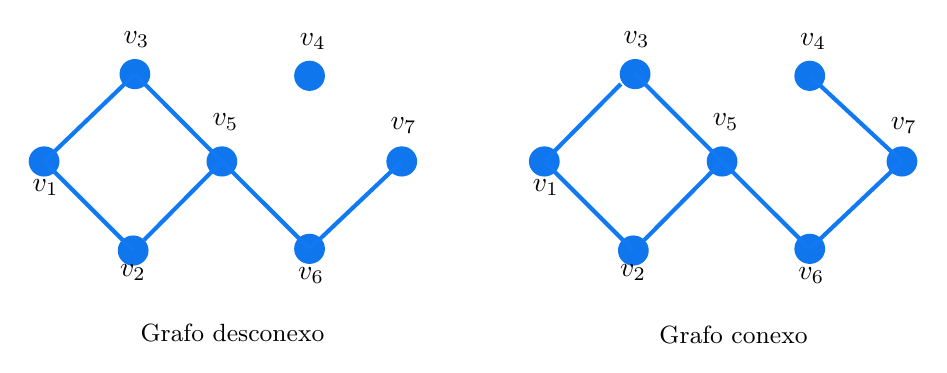
\begin{tikzpicture}[x=0.75pt,y=0.75pt,yscale=-1,xscale=1]
%uncomment if require: \path (0,171); %set diagram left start at 0, and has height of 171

%Shape: Ellipse [id:dp9697628618127521] 
\draw  [draw opacity=0][fill={rgb, 255:red, 15; green, 118; blue, 237 }  ,fill opacity=1 ] (8.01,70.75) .. controls (8.01,66.74) and (11.33,63.48) .. (15.42,63.48) .. controls (19.51,63.48) and (22.83,66.74) .. (22.83,70.75) .. controls (22.83,74.77) and (19.51,78.02) .. (15.42,78.02) .. controls (11.33,78.02) and (8.01,74.77) .. (8.01,70.75) -- cycle ;
%Shape: Ellipse [id:dp5039590702508365] 
\draw  [draw opacity=0][fill={rgb, 255:red, 15; green, 118; blue, 237 }  ,fill opacity=1 ] (50.92,113.67) .. controls (50.92,109.66) and (54.24,106.41) .. (58.33,106.41) .. controls (62.42,106.41) and (65.74,109.66) .. (65.74,113.67) .. controls (65.74,117.69) and (62.42,120.94) .. (58.33,120.94) .. controls (54.24,120.94) and (50.92,117.69) .. (50.92,113.67) -- cycle ;
%Shape: Ellipse [id:dp12129085059451494] 
\draw  [draw opacity=0][fill={rgb, 255:red, 15; green, 118; blue, 237 }  ,fill opacity=1 ] (51.76,28.66) .. controls (51.76,24.64) and (55.08,21.39) .. (59.17,21.39) .. controls (63.26,21.39) and (66.58,24.64) .. (66.58,28.66) .. controls (66.58,32.67) and (63.26,35.93) .. (59.17,35.93) .. controls (55.08,35.93) and (51.76,32.67) .. (51.76,28.66) -- cycle ;
%Shape: Ellipse [id:dp770035428545905] 
\draw  [draw opacity=0][fill={rgb, 255:red, 15; green, 118; blue, 237 }  ,fill opacity=1 ] (93.67,70.75) .. controls (93.67,66.74) and (96.99,63.48) .. (101.08,63.48) .. controls (105.17,63.48) and (108.49,66.74) .. (108.49,70.75) .. controls (108.49,74.77) and (105.17,78.02) .. (101.08,78.02) .. controls (96.99,78.02) and (93.67,74.77) .. (93.67,70.75) -- cycle ;
%Shape: Ellipse [id:dp4278661867814306] 
\draw  [draw opacity=0][fill={rgb, 255:red, 15; green, 118; blue, 237 }  ,fill opacity=1 ] (135.9,112.85) .. controls (135.9,108.83) and (139.22,105.58) .. (143.31,105.58) .. controls (147.4,105.58) and (150.72,108.83) .. (150.72,112.85) .. controls (150.72,116.86) and (147.4,120.12) .. (143.31,120.12) .. controls (139.22,120.12) and (135.9,116.86) .. (135.9,112.85) -- cycle ;
%Shape: Ellipse [id:dp21316118455483957] 
\draw  [draw opacity=0][fill={rgb, 255:red, 15; green, 118; blue, 237 }  ,fill opacity=1 ] (180.33,70.75) .. controls (180.33,66.74) and (183.65,63.48) .. (187.74,63.48) .. controls (191.83,63.48) and (195.15,66.74) .. (195.15,70.75) .. controls (195.15,74.77) and (191.83,78.02) .. (187.74,78.02) .. controls (183.65,78.02) and (180.33,74.77) .. (180.33,70.75) -- cycle ;
%Shape: Ellipse [id:dp051427762117636666] 
\draw  [draw opacity=0][fill={rgb, 255:red, 15; green, 118; blue, 237 }  ,fill opacity=1 ] (135.9,29.48) .. controls (135.9,25.47) and (139.22,22.21) .. (143.31,22.21) .. controls (147.4,22.21) and (150.72,25.47) .. (150.72,29.48) .. controls (150.72,33.5) and (147.4,36.75) .. (143.31,36.75) .. controls (139.22,36.75) and (135.9,33.5) .. (135.9,29.48) -- cycle ;
%Straight Lines [id:da7831429186189045] 
\draw [color={rgb, 255:red, 16; green, 121; blue, 243 }  ,draw opacity=1 ][fill={rgb, 255:red, 0; green, 0; blue, 0 }  ,fill opacity=1 ][line width=1.5]    (15.42,70.75) -- (59.17,28.66) ;
%Straight Lines [id:da7661987549866738] 
\draw [color={rgb, 255:red, 16; green, 121; blue, 243 }  ,draw opacity=1 ][fill={rgb, 255:red, 0; green, 0; blue, 0 }  ,fill opacity=1 ][line width=1.5]    (101.08,70.75) -- (59.17,28.66) ;
%Straight Lines [id:da47492616893819006] 
\draw [color={rgb, 255:red, 16; green, 121; blue, 243 }  ,draw opacity=1 ][fill={rgb, 255:red, 0; green, 0; blue, 0 }  ,fill opacity=1 ][line width=1.5]    (15.42,70.75) -- (58.33,113.67) ;
%Straight Lines [id:da0864666307237163] 
\draw [color={rgb, 255:red, 16; green, 121; blue, 243 }  ,draw opacity=1 ][fill={rgb, 255:red, 0; green, 0; blue, 0 }  ,fill opacity=1 ][line width=1.5]    (63.63,108.56) -- (101.08,70.75) ;
%Straight Lines [id:da503703157006737] 
\draw [color={rgb, 255:red, 16; green, 121; blue, 243 }  ,draw opacity=1 ][fill={rgb, 255:red, 0; green, 0; blue, 0 }  ,fill opacity=1 ][line width=1.5]    (101.08,70.75) -- (143.31,112.85) ;
%Straight Lines [id:da6127732499224423] 
\draw [color={rgb, 255:red, 16; green, 121; blue, 243 }  ,draw opacity=1 ][fill={rgb, 255:red, 0; green, 0; blue, 0 }  ,fill opacity=1 ][line width=1.5]    (143.31,112.85) -- (187.74,70.75) ;
%Shape: Ellipse [id:dp2065636373029469] 
\draw  [draw opacity=0][fill={rgb, 255:red, 15; green, 118; blue, 237 }  ,fill opacity=1 ] (249.01,70.75) .. controls (249.01,66.74) and (252.33,63.48) .. (256.42,63.48) .. controls (260.51,63.48) and (263.83,66.74) .. (263.83,70.75) .. controls (263.83,74.77) and (260.51,78.02) .. (256.42,78.02) .. controls (252.33,78.02) and (249.01,74.77) .. (249.01,70.75) -- cycle ;
%Shape: Ellipse [id:dp6233890933885398] 
\draw  [draw opacity=0][fill={rgb, 255:red, 15; green, 118; blue, 237 }  ,fill opacity=1 ] (291.92,113.67) .. controls (291.92,109.66) and (295.24,106.41) .. (299.33,106.41) .. controls (303.42,106.41) and (306.74,109.66) .. (306.74,113.67) .. controls (306.74,117.69) and (303.42,120.94) .. (299.33,120.94) .. controls (295.24,120.94) and (291.92,117.69) .. (291.92,113.67) -- cycle ;
%Shape: Ellipse [id:dp44560216059762725] 
\draw  [draw opacity=0][fill={rgb, 255:red, 15; green, 118; blue, 237 }  ,fill opacity=1 ] (292.76,28.66) .. controls (292.76,24.64) and (296.08,21.39) .. (300.17,21.39) .. controls (304.26,21.39) and (307.58,24.64) .. (307.58,28.66) .. controls (307.58,32.67) and (304.26,35.93) .. (300.17,35.93) .. controls (296.08,35.93) and (292.76,32.67) .. (292.76,28.66) -- cycle ;
%Shape: Ellipse [id:dp023538341517420847] 
\draw  [draw opacity=0][fill={rgb, 255:red, 15; green, 118; blue, 237 }  ,fill opacity=1 ] (334.67,70.75) .. controls (334.67,66.74) and (337.99,63.48) .. (342.08,63.48) .. controls (346.17,63.48) and (349.49,66.74) .. (349.49,70.75) .. controls (349.49,74.77) and (346.17,78.02) .. (342.08,78.02) .. controls (337.99,78.02) and (334.67,74.77) .. (334.67,70.75) -- cycle ;
%Shape: Ellipse [id:dp09979920722283486] 
\draw  [draw opacity=0][fill={rgb, 255:red, 15; green, 118; blue, 237 }  ,fill opacity=1 ] (376.9,112.85) .. controls (376.9,108.83) and (380.22,105.58) .. (384.31,105.58) .. controls (388.4,105.58) and (391.72,108.83) .. (391.72,112.85) .. controls (391.72,116.86) and (388.4,120.12) .. (384.31,120.12) .. controls (380.22,120.12) and (376.9,116.86) .. (376.9,112.85) -- cycle ;
%Shape: Ellipse [id:dp16504719377994537] 
\draw  [draw opacity=0][fill={rgb, 255:red, 15; green, 118; blue, 237 }  ,fill opacity=1 ] (421.33,70.75) .. controls (421.33,66.74) and (424.65,63.48) .. (428.74,63.48) .. controls (432.83,63.48) and (436.15,66.74) .. (436.15,70.75) .. controls (436.15,74.77) and (432.83,78.02) .. (428.74,78.02) .. controls (424.65,78.02) and (421.33,74.77) .. (421.33,70.75) -- cycle ;
%Shape: Ellipse [id:dp6060581993847338] 
\draw  [draw opacity=0][fill={rgb, 255:red, 15; green, 118; blue, 237 }  ,fill opacity=1 ] (376.9,29.48) .. controls (376.9,25.47) and (380.22,22.21) .. (384.31,22.21) .. controls (388.4,22.21) and (391.72,25.47) .. (391.72,29.48) .. controls (391.72,33.5) and (388.4,36.75) .. (384.31,36.75) .. controls (380.22,36.75) and (376.9,33.5) .. (376.9,29.48) -- cycle ;
%Straight Lines [id:da8167669030114226] 
\draw [color={rgb, 255:red, 16; green, 121; blue, 243 }  ,draw opacity=1 ][fill={rgb, 255:red, 0; green, 0; blue, 0 }  ,fill opacity=1 ][line width=1.5]    (256.42,70.75) -- (293.28,33.45) ;
%Straight Lines [id:da20942586645429806] 
\draw [color={rgb, 255:red, 16; green, 121; blue, 243 }  ,draw opacity=1 ][fill={rgb, 255:red, 0; green, 0; blue, 0 }  ,fill opacity=1 ][line width=1.5]    (342.08,70.75) -- (300.17,28.66) ;
%Straight Lines [id:da3053611119523447] 
\draw [color={rgb, 255:red, 16; green, 121; blue, 243 }  ,draw opacity=1 ][fill={rgb, 255:red, 0; green, 0; blue, 0 }  ,fill opacity=1 ][line width=1.5]    (256.42,70.75) -- (299.33,113.67) ;
%Straight Lines [id:da5742069377153007] 
\draw [color={rgb, 255:red, 16; green, 121; blue, 243 }  ,draw opacity=1 ][fill={rgb, 255:red, 0; green, 0; blue, 0 }  ,fill opacity=1 ][line width=1.5]    (304.63,108.56) -- (342.08,70.75) ;
%Straight Lines [id:da21404193811759664] 
\draw [color={rgb, 255:red, 16; green, 121; blue, 243 }  ,draw opacity=1 ][fill={rgb, 255:red, 0; green, 0; blue, 0 }  ,fill opacity=1 ][line width=1.5]    (342.08,70.75) -- (384.31,112.85) ;
%Straight Lines [id:da8949010675644655] 
\draw [color={rgb, 255:red, 16; green, 121; blue, 243 }  ,draw opacity=1 ][fill={rgb, 255:red, 0; green, 0; blue, 0 }  ,fill opacity=1 ][line width=1.5]    (384.31,112.85) -- (428.74,70.75) ;
%Straight Lines [id:da9183865181036905] 
\draw [color={rgb, 255:red, 16; green, 121; blue, 243 }  ,draw opacity=1 ][fill={rgb, 255:red, 0; green, 0; blue, 0 }  ,fill opacity=1 ][line width=1.5]    (384.31,29.48) -- (428.74,70.75) ;

% Text Node
\draw (8.43,77.78) node [anchor=north west][inner sep=0.75pt]    {$v_{1}$};
% Text Node
\draw (50.5,119.05) node [anchor=north west][inner sep=0.75pt]    {$v_{2}$};
% Text Node
\draw (52.18,6.8) node [anchor=north west][inner sep=0.75pt]    {$v_{3}$};
% Text Node
\draw (137.16,7.62) node [anchor=north west][inner sep=0.75pt]    {$v_{4}$};
% Text Node
\draw (95.09,46.42) node [anchor=north west][inner sep=0.75pt]    {$v_{5}$};
% Text Node
\draw (136.32,120.51) node [anchor=north west][inner sep=0.75pt]    {$v_{6}$};
% Text Node
\draw (180.91,48.07) node [anchor=north west][inner sep=0.75pt]    {$v_{7}$};
% Text Node
\draw (60.39,147.44) node [anchor=north west][inner sep=0.75pt]  [font=\small] [align=left] {Grafo desconexo};
% Text Node
\draw (249.43,77.78) node [anchor=north west][inner sep=0.75pt]    {$v_{1}$};
% Text Node
\draw (291.5,119.05) node [anchor=north west][inner sep=0.75pt]    {$v_{2}$};
% Text Node
\draw (293.18,6.8) node [anchor=north west][inner sep=0.75pt]    {$v_{3}$};
% Text Node
\draw (378.16,7.62) node [anchor=north west][inner sep=0.75pt]    {$v_{4}$};
% Text Node
\draw (336.09,46.42) node [anchor=north west][inner sep=0.75pt]    {$v_{5}$};
% Text Node
\draw (377.32,120.51) node [anchor=north west][inner sep=0.75pt]    {$v_{6}$};
% Text Node
\draw (421.91,48.07) node [anchor=north west][inner sep=0.75pt]    {$v_{7}$};
% Text Node
\draw (310.39,148.44) node [anchor=north west][inner sep=0.75pt]  [font=\small] [align=left] {Grafo conexo};


\end{tikzpicture}